\documentclass{scu-thesis}

% Some very useful LaTeX packages
\usepackage{times}	% for using the Times-Roman font
\usepackage[pdftex]{graphicx} % Used to include figures and pictures in the article
% declare the path(s) where your graphic files are
\graphicspath{{./img/}{./figures/}}
% and their extensions so you won't have to specify these with
% every instance of \includegraphics
\DeclareGraphicsExtensions{.pdf,.jpeg,.png}
\usepackage{amsmath, amsthm, amsfonts, amssymb, amsxtra, amsopn} % Math
\usepackage{algorithm} % Used for writing algorithms in an article
\usepackage[noend]{algpseudocode} % Allows psuedocode keywords (e.g., "if", "while", "for", etc.) in algorithms.
\usepackage{multirow,array} % Matrices and multi-line number structures
\usepackage[export]{adjustbox} % Also loads graphicx if not already loaded
\usepackage{epsfig} % Allow postscript graphics files
\usepackage{float} % Manage floats
\usepackage{tabularx, booktabs, longtable, booktabs, makecell} % Tables
\usepackage{xcolor, colortbl} % Used for coloring text and the cells of tables
\usepackage{cmap} % Build character maps for generated PDF files
\usepackage{textcomp} % Required for upquote
\usepackage{listings} % Used for printing source code in articles
\usepackage[shortcuts]{extdash} % Allow the use of unbreakable "extdash" spacers.
\usepackage{enumitem} % Manage item lists
% Do not add extra space around itemizes
\setlist[itemize]{noitemsep, topsep=0pt}
% Right-aligned column in tabularx
\newcolumntype{Y}{>{\raggedleft\arraybackslash}X}
% Set the file name for the acknowledgments page file.
\acknowledgments{acknowledgments}
% Set the file name for the dedication page file.
\dedication{dedication}



% These must be set first ... the rest of the thesis commands rely on them.
\author{Noah Tall}
\author{Mae Bea Wright}
\title{On the Construction of Matter, or Is There a God Particle?}
\department{Department of Molecular Engineering}
\department{Department of Religious Studies}
\degree{Bachelor of Science in Molecular Engineering}
\degree{Bachelor of Arts in Transcendental Meditation}
% Only bachelor's theses should have multiple authors and/or be from
% multiple departments.  Signatures required:
%
% Bachelor's theses: advisor(s), department chair(s)
% Master's theses: advisor, reader, department chair
% Doctoral theses: doctoral committee (including advisor), department chair


% Specify new custom commands
\newcommand{\norm}[1]{\left\lVert#1\right\rVert}
\renewcommand{\vec}[1]{\mathbf{#1}}
\def\eg{\emph{e.g.}}



% Document starts here
\begin{document}
\frontmatter
\signature{Thesis Advisor}
\signature{Thesis Advisor}
\signature{Department Chair}
\signature{Department Chair}

\maketitle
\begin{abstract}
A good abstract is a concise summary (1--2 paragraphs) of the entire
project: introduction, problem statement, work accomplished, results,
conclusions, and recommendations. When you write the abstract, imagine
that the reader will not read anything else, but that you must get
your major point across immediately. This requires efficiency of words
and phrases. An abstract is written to stand alone, without jargon or
reference to figures and tables in the report body.
\end{abstract}

\acknowledgementpage   %% this is optional and can be commented out
% \dedicationpage        %% this is optional and can be commented out

\tableofcontents
\listoffigures

\mainmatter
\chapter{Introduction}

\section{Motivation}

This document is a LaTeX template created by David C. Anastasiu for thesis and project report authors from the College of Science and Engineering (CSEN) at Santa Clara University (SCU). The template extends an initial LaTeX class created by Prof. Darren Atkinson and attempts to simplify the formatting of theses for students while also guiding them in the writing process. Students should, however, read the current library thesis style requirements carefully and rectify any style discrepancies before submitting their theses. Additionally, note that reviewers are very strict on grammar and spelling mistakes.


\section{Solution}

The present ``thesis'' serves as a visual example of what the finished thesis product should look like. In addition, it provides some guidance on how to use the scu-thesis style, the provided LaTeX template project, and LaTeX in general to produce a quality thesis that complies with submission requirements. LaTeX, in combination with the provided style, automate many of the style aspects of the thesis, as long as students do not modify the style or introduce new style elements manually in the text. For example, one can make all section titles bold by simply putting the text within a \texttt{{\textbackslash}textbf} block. However, that would break the style and cause the thesis to be returned for edits by the reviewers. Students are thus, once again, urged to refrain from style modifications and to double-check style compliance against the style guide before submitting their theses.

Throughout the thesis, we will make use of tables and figures from some of my own papers and my students' theses. These tables and figures will likely be taken out of context and should not be considered relevant to the topic of this thesis. They are simply provided as examples for how to properly include these elements in a thesis document.

The remainder of this thesis is structured as follows. First, in Chapter~\ref{ch:literature_review}, we will introduce the reader to the task of reviewing literature that is relevant to the chosen topic of study, with the goal of identifying the current state-of-the-art method or system that potentially solves the problem at hand. This is the basis of all research projects, as we should not ``re-invent the wheel'' and try not to repeat mistakes made by others. Chapter~\ref{ch:methods} serves as a brief introduction to writing documents in the TeX macro language. Additional example chapters are included for reference and should be edited/changed as necessary for your thesis/project. Finally, Chapter~\ref{ch:future_work} describes to-do items envisioned for this project and Chapter~\ref{ch:conclusion} concludes this thesis.
\chapter{Literature Survey}\label{ch:literature_review}

\section{How to Write a Literature Review}\label{sec:literature_review:howto}

This chapter will contain some practical advice for starting the research journey by finding the state-of-the-art for the project at hand. However, until we have time to write this chapter, we are including some related works form an in-progress project.

In this chapter, we review some supervised and unsupervised techniques that are used to identify human activities using mobile sensor data. Additionally, we review some methods that can help identify appropriate features that need to be extracted from the raw sensor data to better identify activity patterns.

\subsection{Activity Recognition}
Appropriate datasets are hard to find for human activity recognition (HAR) research, which lead many authors to collect their own data using several sensors. Chen and Shen~\cite{chen2017} presented performance analysis based on the placement of smartphones on various parts of a subject's body. In their data collection phase, they captured data from a combination of different sensors, e.g., only accelerometer versus combined accelerometer and gyroscope, from smartphones attached to the forearm, abdomen, or legs of the subject, with the ultimate goal of classifying the type of activity being performed.
%%
Su et al.~\cite{su2014} computed features in two different domains: time and frequency. In the time domain, they calculated mean, max-min, standard deviation, correlation, and signal magnitude area (SMA). In the frequency domain, they calculated energy, entropy, binned distribution, and the time difference between peaks. They tested a number of supervised learning methods for activity recognition, such as using decision tree, na\"{i}ve Bayes, and support vector machine (SVM) classification models. 

% \subsection{Supervised Approaches}
Anguita et al.~\cite{anguita2013} focused on labeled data collection using built-in smartphone sensors (accelerometer, gyroscope at 50Hz) with six predefined activity labels. To validate the quality of the dataset, they used the SVM classifier, after filtering noise, and feature mapping to a randomly-split test/train dataset. Kim et al.~\cite{kim2010} summarized pattern discovery in supervised HAR approaches, including hidden Markov model (HMM), linear chain conditional random fields (CRF), and skip-chain CRF (SCCRF).
% \subsection{Unsupervised Approaches}
Several approaches have been devised for unsupervised learning for human activity recognition. Bhattacharya et al.~\cite{bhattacharya2014} and Li et al.~\cite{yongmou2014} compared sparse encoding and principle component analysis (PCA) for activity recognition from unlabeled sensor data and found sparse encoding to be better. In~\cite{yongmou2014}, Li et al. also compared denoising autoencoder (DAE) and fast fourier transform (FFT) techniques for feature extraction and found sparse autoencoder to provide better results than other techniques.

Chamroukhi et al.~\cite{chamroukhi2013} described a method to identify hidden discrete logistic processes that maximize the likelihood of data being observed, which they trained via a dedicated expectation maximization (EM) algorithm. Similarity, Kwon et al.~\cite{kwon2014} compared various clustering algorithms for labeling a mixed bag of known and unknown activities. Results showed that given a number of activities, GMM seems to outperform $k$-means and hierarchical clustering for a given known number of activities, but DBSCAN~\cite{ester1996} proved the best choice when the number of activities is unknown.

Wang et al.~\cite{wang2014} discussed linear dynamical systems for human activity recognition, which uses $k$-medoids clustering and a bag-of-systems (BoS) to predict activities involving motion, such as jumping and running. Ronao and Cho~\cite{ronao2015} proposed using a deep convolutional neural networks (DCNN) to extract features from the time series data. They found that, as the number of layers increases, the classification performance improved but the complexity of derived features decreased. Analysis of additional algorithms showed that DCNNs with hand designed features yield better results. Gjoreski and Roggen~\cite{gjoreski2017} proposed a method called ``Unsupervised Online Activity Discovery Using Temporal Behavior Assumption'' (UnADevs) based on an online clustering which includes the temporal information of the occurring activities. It is well suited to identify clusters of repeating activities while keeping track of the time interval of discovered activity clusters.

Most of the works in the area of human activity recognition involves smartphones, which have many built-in sensors  which can generate diverse signal shapes given the phone's position. These signals can be used to recognize many different human activities. Existing works have used many different combinations of the sensors and machine learning techniques, but are primarily focused on identifying base activities (sitting, running), while our method is designed to characterize human activity patterns and identify how these patterns change over time.

\subsection{Multivariate Time Series Segmentation}
Time series segmentation has been an area of interest for many research communities, including signal processing, pattern recognition, machine learning and language processing. 
% Time series segmentation with multi-variables adds new challenges to segment definition. Many have introduced approaches like statistical latent processing models, clustering algorithms, dynamic programming to likely address the segmentation issue in different fields. 
%
Abonyi et al.~\cite{abonyi2005} presented fuzzy clustering as one such approach but it requires clusters to be contiguous in time. It uses probabilistic PCA models to measure homogeneity of the segments and fuzzy sets. To overcome this limitation, Wang et al. proposed an improved unsupervised method~\cite{wang2012} that can automatically determine the optimal segmentation order. 

Dynamic programming (DP) algorithms have been widely explored to automatically segment multivariate time series~\cite{guo2015, anastasiu2015}. 
% The advantage is that it can recursively formulate segmentation errors of univariate time series to multivariate time series. Hence making dynamic programming a computationally viable approach for this problem. 
In one example, Anastasiu et al.~\cite{anastasiu2015} proposed an algorithm for optimal cross-user segmentation for identifying how users use their computers and how that usage changes over time. Our method is similar in scope, but focused on automatic discovery of human activity patterns. A similar dynamic programming based approach was proposed by Guo et al.~\cite{guo2016}. It initially applies fuzzy clustering to predefined segments and uses dynamic time warping to determine distances between non-equal length series. Segments are then iteratively updated through a segmentation objective function optimized using dynamic programming.

% Majority of the above works focus on activity detection based on various sensors, data collection methods and, supervised/unsupervised models. A handful of research have also gone into time series segmentation in various domains. In this project, we propose to implement a multivariate time-series segmentation on human activities data collected over time, to classify activity patterns for a group of users.

\subsection{Where to Find More Information About Literature Reviews}\label{sec:literature_review:more_info}

This section will contain some relevant references on this topic.
\chapter{Methods}\label{ch:methods}

\section{Mini-introduction to LaTeX}\label{sec:latex}

This chapter needs to be filled out. For now, it contains some very basic examples.


\subsection{Equations}\label{sec:latex:equations}

Equations and mathematical formulas can be included in-line, within the text, for example when explaining that $\norm{\vec x}_2$ signifies the $\ell_2$ norm of a vector, as long as the included math formula or symbols are short (less than half a line). For longer formulas, or formulas that need to be referenced later in the text, one should use the \texttt{equation} macro or related macros, e.g., \texttt{align}. For example, the dot-product of two vectors, $\vec x$ and $\vec y$, is defined as
\begin{equation}\label{eq:dot-product}
    \langle \vec x, \vec y \rangle = \vec{x}^T\vec{y} = \sum_{j=1}^m x_j\times y_j.
\end{equation}

Note that equations can be assigned labels and referenced throughout the text. However, unlike figures and tables (see next sections), the equation should be defined prior to its reference. Now that we can defined the formula for the vector dot-product, we can now refer to Equation~\ref{eq:dot-product} to remind readers of its definition.

\subsection{Figures}\label{sec:latex:figures}

Figures should contain a caption at the bottom. The caption is a sentence or phrase that describes the content of the figure. As such, it should start with a capital letter and end with a period. The caption is not a title, so subsequent words after the first word should not be capitalized unless they are proper names. A figure should be introduced in the text prior to its inclusion in the text. When referring to the figure, make use of the  \texttt{{\textbackslash}figurename} macro, provided by the IEEE style, to ensure style compliance. Additionally, use a non-breaking space character to connect the \figurename~text with the number assigned to the figure reference. This will ensure that \figurename~and the reference will be included on the same line. For example, \figurename~\ref{fig:proj-arch} introduces our project architecture. Note that font sizes in figures and tables may be smaller than the rest of the thesis. However, they should be readable.

\begin{figure}[!htb]
  \centering
  \includegraphics[width=0.7\textwidth]{img/proj-arch.pdf}
  \caption{Project architecture.}
  \label{fig:proj-arch}
\end{figure}


\subsection{Tables}\label{sec:latex:tables}

Tables should contain a caption at the top. Unlike figures, the caption in the table is the table title, and it should be capitalized accordingly. The table should be presented in the text prior to its inclusion in the text. Moreover, references to tables should follow the same directions as those for figures, except use the \texttt{{\textbackslash}tablename} macro. For example, \tablename~\ref{tbl:dataset} introduces statistics about the dataset used in our analysis.

\begin{table}[!htb]
\caption{Dataset Characteristics}
\label{tbl:dataset}
\centering
\begin{tabular}{c|c|c|c|c|c}
\hline
\textbf{Name} & \textbf{Duration (h)} & \textbf{Activities} & \textbf{Subjects}  & \textbf{Sensors} & \textbf{Frequency (Hz)} \\ 
\hline
JSI-ADL & 18.8 & 14 & 10 & 2 & 50\\ 
REALDISP & 9 & 33 & 17 & 2 & 50\\ 
UCI-HAR & 1.5 & 6 & 30 & 2 & 50\\ 
Ours & 1500 & 14 & 24 & 2 & 20\\ 
\hline
\end{tabular}
\end{table}

\subsection{Algorithms}\label{sec:latex:algorithms}

LaTeX provides powerful macros for writing algorithms. Note that labels can be included within the algorithm, which allows the writer to refer to specific lines in the algorithm. The algorithm should be introduced first. Note that the label referring to the whole algorithm is placed right after the caption. Similar to a table, the caption is a title and should be capitalized accordingly. For example, Algorithm~\ref{alg:proj-motif} describes the process for producing a normalized 2-hop left-projection of a bipartite graph described by the vertex sets $V^1$ and $V^2$ and the edge set $E$. Long algorithms (greater than half a page) should be relegated to the Appendix.

\begin{algorithm}[!htb]
\caption{The Normalized 2-hop Left-Projection Algorithm}\label{alg:proj-motif}
\small
\begin{algorithmic}[1]
\Procedure{Project}{$V^1,V^2,E$}\Comment{Construct the left projection $G^1$}
%%
\item[] \quad\; // Initialize and compute degree vectors.
\For {$(v^1_i, v^2_j) \in E$} \Comment{Count neighbors}
\State $\lambda_n(i) \gets \lambda_n(i) + 1$
\State $\lambda_m(j) \gets \lambda_m(j) + 1$
\EndFor
\item[] \quad\; // SpGEMM
%%
\For {$v^1_i \in V^1$} \label{alg:proj-motif-spgemm1}
\State $acc(:) \gets 0$ \Comment{Initialize output row accumulator data structure}
\For {$v^2_k \in \Gamma(v^1_i)$}
\State $l \gets  (1/\lambda_n(i)) \times \times w_{i,k} \times (1/\lambda_m(k))$ \label{alg:proj-motif-lk}
\For {$v^1_j \in \Gamma(v^2_k)$}
\If {$v^1_j \ne v^1_i$} \Comment{Avoid computing output diagonal}
\State $acc(j) \gets acc(j) + l \times w_{j,k}$ \label{alg:proj-motif-accum}
\EndIf
\EndFor
\EndFor
\State $C(i,:) = acc(:)$
\EndFor\label{alg:proj-motif-spgemm2}
\item[] \quad\; // Normalize rows of $C$
%%
\For {$i = 1, \ldots, |V^1|$}\label{alg:proj-motif-norm1}
\State $n_i \gets 0$
\For {$j = 1, \ldots, |V^2| \text{ s.t. } C(i,j) > 0$}
\State $n_i \gets n_i + \text{abs}(C(i,j))$
\EndFor
\For {$j = 1, \ldots, |V^2| \text{ s.t. } C(i,j) > 0$}
\State $C(i,j) \gets C(i,j) / n_i$
\EndFor
\EndFor\label{alg:proj-motif-norm2}
\State \textbf{return} $C$\Comment{Edge set weight matrix for $G^1$}
\EndProcedure
\end{algorithmic}
\end{algorithm}

After introducing the algorithm, one can then refer to sections of the algorithm in the process of describing it in the text. For example, note that line~\ref{alg:proj-motif-accum} denotes the accumulation of projection weights for a vertex $v_i^1$ in $V^1$. For theses that contain many mathematical symbols, it is a good idea to provide the reader with a reference for the meaning of these symbols. This table is generally included in the preliminary chapters, after the introduction. We will include an example here. \tablename~\ref{tbl:notation-g} provides a reference for notation used throughout the paper that the algorithm above is included in.

\begin{table}[!htb]
\caption {Graph and Projection Notation} \label{tbl:notation-g}
\centering
\small
 \begin{tabular}{l l}
 \hline
 \textbf{Symbol} & \textbf{Meaning} \\ 
 \hline
 $G$ & A graph topology. \\
 $V^1$, $V^2$ & The left and right node partitions in a bipartite graph. \\
 $E$ & The set of edges in $G$. \\
 $|X|$ & The cardinality of set $X$. \\
 $v^1_i \in V^1$ & A vertex in the left node partition $V^1$. \\
 $v^2_j \in V^2$ & A vertex in the right node partition $V^2$. \\
 $(v^1_i, v^2_j, w_{i,j})\in E$ & The edge connecting nodes $v^1_i$ and $v^2_j$ with weight $w_{i,j}$ in graph $G$. \\
 $\Gamma(v^1_i)$ & The set of vertices in $V^2$ adjacent to $v^1_i$, i.e., its neighborhood. \\
 $\lambda_n,\lambda_m$ & Node degree vectors for the left and right partitions.\\
 $A \in \mathbb{R}^{n\times m}$ & The edge weight matrix for the bipartite graph $G$; $A(i,j) = w_{i,j}$. \\
 $B$ & Weighted adjacency matrix for graph $G$.\\
 \hline
 $G^1 = (V^1, E^1)$ & The left projection graph.\\
 $G^2 = (V^2, E^2)$ & The right projection graph.\\
 $G^b = (V, E^b)$ & The biprojection graph.\\
 $(v^1_i, v^1_j, s^1_{i,j})\in E^1$ & The edge connecting $v^1_i$ and $v^1_j$ with weight $s^1_{i,j}$ in the left projection graph. \\
 $W^1$ & Edge weight matrix for the left projection graph; $W^1(i,j) = s^1_{i,j}$.\\
 $W^2$ & Edge weight matrix for the right projection graph; $W^2(i,j) = s^2_{i,j}$.\\
 $W$ & Weighted adjacency matrix for the bi-projection graph of $G$.\\
 \hline
 \end{tabular}
\end{table}

\subsection{Location of Floats}\label{sec:latex:floats}

Floats (e.g., algorithms, tables and figures) should not follow the IEEE standard of being placed at the top or bottom of the page. In a thesis, they must appear right after their reference and not break any paragraphs, i.e., they should be placed in the text, after the paragraph in question. Use the location hint \texttt{[!htb]} to let LaTeX know the float should be placed in between paragraphs. If the float takes up an entire page and the last paragraph on the current page does not fit in its entirety, it should be moved after the float page to avoid breaking the continuity of the paragraph, leaving some blank lines at the end of the current page.

Pages that contain only floats will have floats vertically centered, which will produce additional blank lines between the floats in the page or between a float and the top and bottom of the page. The thesis guidelines specifically prohibit additional white space in the thesis. This case and the one discussed in the previous paragraph are the only acceptable reasons for having extra blank lines in the text.

\subsection{Citations}\label{sec:latex:citations}
When citing papers, it is advisable to collect BibTeX records for the papers that you wish to cite, which will be automatically processed into the correct citation style by the LaTeX/BibTeX compiler. Citing a work by Anastasiu and Karypis~\cite{anastasiu-dsaa2016}, for example, is as simple as writing ``Anastasiu and Karipis\textasciitilde{\textbackslash}cite\{anastasiu-dsaa2016\},'' where \textit{anastasiu-dsaa2016} is the key associated with the paper's BibTeX record in the \textit{references.bib} file. Note the non-breaking space character (\textasciitilde) between the word before the citation and the \textit{{\textbackslash}cite} command. It gets translated into a space, and does not allow LaTeX to print the citation on a different line than the connecting word. This, of course, does not work if you put a space between the word and the non-breaking space character, e.g., ``Karypis \textasciitilde{\textbackslash}cite\{anastasiu-dsaa2016\}''.

When citing papers with a single author, one should refer to the work by citing the author's last name. For example, Anastasiu~\cite{anastasiu-idsc2017} used a combination of heuristic candidate selection and search space filtering to efficiently identify approximate nearest neighbors. When the work has two authors, both authors should be referenced by their last name, as in the previous example of the work by Anastasiu and Karypis~\cite{anastasiu-dsaa2016}. Finally, if there are more than two authors, one should reference the first author's last name, followed by the phrase \textit{et al.}, which is short for the Latin \textit{et alia} and means ``and others''. Note the placement of the period. As an example, Kapoor et al.~\cite{kapoor-fie2018} discuss the benefits of competitive active learning in engineering education. Note that it is not necessary to mention authors by last name when listing multiple works as examples or evidence of a statement. For example, many recent works have developed filtering-based methods for nearest neighbor graph construction~\cite{anastasiu-icde2014, anastasiu2015, anastasiu-sc2015, anastasiu-sc2016}.


\chapter{Evaluation}

\section{Experimental Design}

\subsection{Data Sets}


\subsection{Evaluation Metrics}


\subsection{Execution Environment}


\section{Experimental Results}


\subsection{Effectiveness Results}



\subsection{Efficiency Results}



\chapter{Future Work}\label{ch:future_work}

\chapter{Societal Issues}\label{ch:societal_issues}

If you do not think an issue, such as ethics for example, has any relation to your project, you can say so, but you should justify this. These responses need not be lengthy, but you should say something about each of the following issues:

\paragraph{Ethical.}
Ethical conduct is what one ought to do in working with others. It is the right thing to do, the moral action. It is not surprising that virtually all of our professional societies and groups, in all professions, have codes of ethical conduct. Professions realize that there are good and bad ways of working with others, and we need to make the distinction. Sometimes it can be difficult to know what is the right thing to do. What ethical questions were or could be raised about your project?

\paragraph{Social.}
Engineering is done within a social context, within a community of other people. Sometimes that community is defined very narrowly, sometimes very broadly. A focus on social issues allows us to consider the impact of our work on society. If we develop this product, or implement this system, what will be the effect? All of our human developments, in engineering and elsewhere, have unanticipated consequences, some good, some bad. We have an obligation to reflect on these consequences as well as we are able.

\paragraph{Political.}
Many of our projects are very political in nature, requiring us to take into consideration the will of the general public, usually through elected representatives. Engineers who work on public projects need to understand the political processes that make such work possible. What is the potential impact of your project or this type of project on society?

\paragraph{Economic.}
Economic considerations in engineering concern the costs of the various steps in the project. Such costs are usually dependent on the engineering decisions that are made during the design phase. Alternative approaches may offer cost options. We also need to consider the cost of money. How do we pay for the cost of a product development? If we must borrow significant amounts of money how do we account for the cost of the loan in the pricing of the product? What economic considerations arose in your project?

\paragraph{Health and Safety.}
We develop our products for the use of the public. Hence we must consider health and safety issues related to our product. How safe does a product have to be? Are there laws that determine this? Are there related ethical issues? What health effects are relevant? What health and safety issues arose in your project?

\paragraph{Manufacturability.}
Manufacturability issues are of great importance. Can the product be built? Is there an easier way to build this product than first imagined? What development time issues arise? What are the cost issues? Could your project be manufactured? What problems might arise?

\paragraph{Sustainability.}
Sustainability means two things in engineering; one is a narrow sense, one broad sense. In the former sense sustainability refers to the degree to which a product that is developed can continue to be viable and useful for a reasonable amount of time. A product that fails soon after it is built and cannot be repaired or updated or modified to fit new needs is not a sustainable product. In the broader sense a community or region or a world, perhaps, that uses its resources effectively so that it can sustain its life for a long time is said to be sustainable. We say that such a community has a sustainable economy. Engineering can help develop sustainable economies. What sustainability issues arise?

\paragraph{Environmental Impact.}
All of our products and systems have some environmental impact, in the uses of valuable resources, or in the production of pollution, or in other changes in our surroundings. The engineer is obliged to consider such impacts, and to point them out where they arise, or are a threat. What are the environmental issues related to your product?

\paragraph{Usability.}
Usability refers to what is sometimes called ``user-friendliness.'' Is the device straightforward, easily learned and easily used by the end user. Is your product usable?

\paragraph{Lifelong learning.}
Lifelong learning is a necessary part of all professions. You wouldn't want to have a doctor who did not know the latest procedures and medications to protect your life. And you wouldn't want an engineer who didn't know the analysis tools that had been developed since graduation, or the cost-effective materials that had just come along. We just have to keep up. Learning never stops. Did this project help prepare you for the time when you will have to learn on your own, or did it inspire you to study new material?

\paragraph{Compassion.}
One definition for compassion is an awareness of and sympathy for the suffering of another. Compassion means to recognize the suffering of another. But let’s look at a broader definition. Let’s define compassion as “the awareness of and sympathy for the suffering of another, and the desire to relieve that suffering.” What does that have to do with engineering? Simple! One of the things that engineers can choose to do in life is to look for and try to relieve suffering where they find it. Perhaps it means replacing an ancient water supply system that is leading to disease in some tiny village, or designing a communication system to protect seniors with illnesses, or designing prosthetic devices for crippled children. Even if we do not decide to make the relieving of suffering the focus of our life’s work, it is still critically important to our fullness as a human being that we feel compassion for the suffering. It is a part of the education that we hope you acquired at Santa Clara.
\chapter{Conclusion}\label{ch:conclusion}

\section{What We Have Learned}


\section{Why it is Important}

\backmatter
%%%%%
%% Appendices are optional. 
%% If none are present, comment out "%%%%%
%% Appendices are optional. 
%% If none are present, comment out "%%%%%
%% Appendices are optional. 
%% If none are present, comment out "\include{appendices}" in main.tex
%%%%%
\appendix
\renewcommand{\thesubsection}{\Alph{subsection}}

\chapter{What Should Be Included in Appendices}\label{apx:appendix1}

Appendices should contain information that is too lengthy to be included in the thesis chapters but further support the conclusions of the thesis. For example, one could include additional experimental results in the form of tables or additional figures. Each appendix should start with a paragraph introducing the items being presented. Additionally, each table or figure should be preceded by a paragraph that explains the data being presented and the conclusions that can be drawn from them. Please note that data already presented in the main thesis should not be repeated in an appendix. One cannot, for example, include the results of an experiment as a figure in the thesis and again as a table in the appendix. One can, however, include detailed results in tables in the appendix and a summary figure in the thesis portraying only the ``best" results.

\section{Subsections in Appendices}\label{apx:appendix1:subsections}

It is possible, and advisable, to use (multiple levels of) subsections in an Appendix. The main Appendix sections may be optionally titled. They will automatically be assigned Appendix A, Appendix B, etc. If a title is present, it will appear on the next line in the appendix and on the same line in the TOC. Sub-sections will be listed in the TOC as A.1, A.2, etc.

Figures, such as \figurename~\ref{fig:nonzero-distr}, should only be referenced in the appendix. The thesis content can point to an appendix but not specifically reference a table or figure in the appendix.

\begin{figure}[!htb]
  \centering
  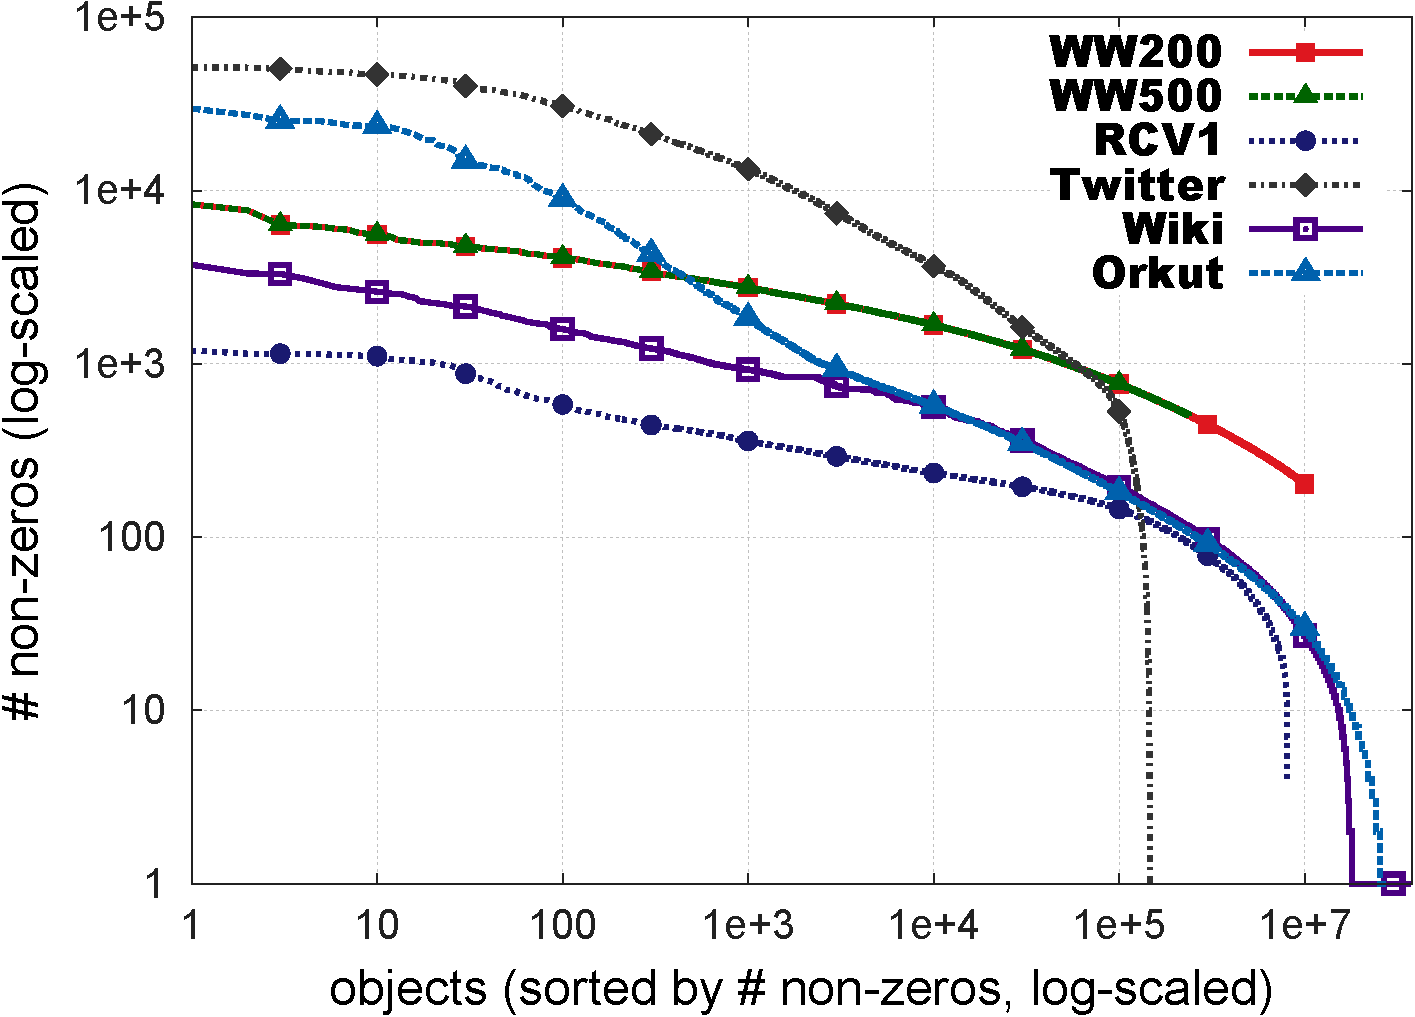
\includegraphics[width=0.6\textwidth]{img/hist-rows.pdf}
  \caption{Distribution of sample non-zeros.}
  \label{fig:nonzero-distr}
\end{figure}


\chapter{Title of Another Appendix}\label{apx:appendix2}

Different appendices should cover unrelated topics. If the appendices are on the same topic, they should just be sub-sections within the same appendix. 

\begin{figure}[tbh]
  \centering
  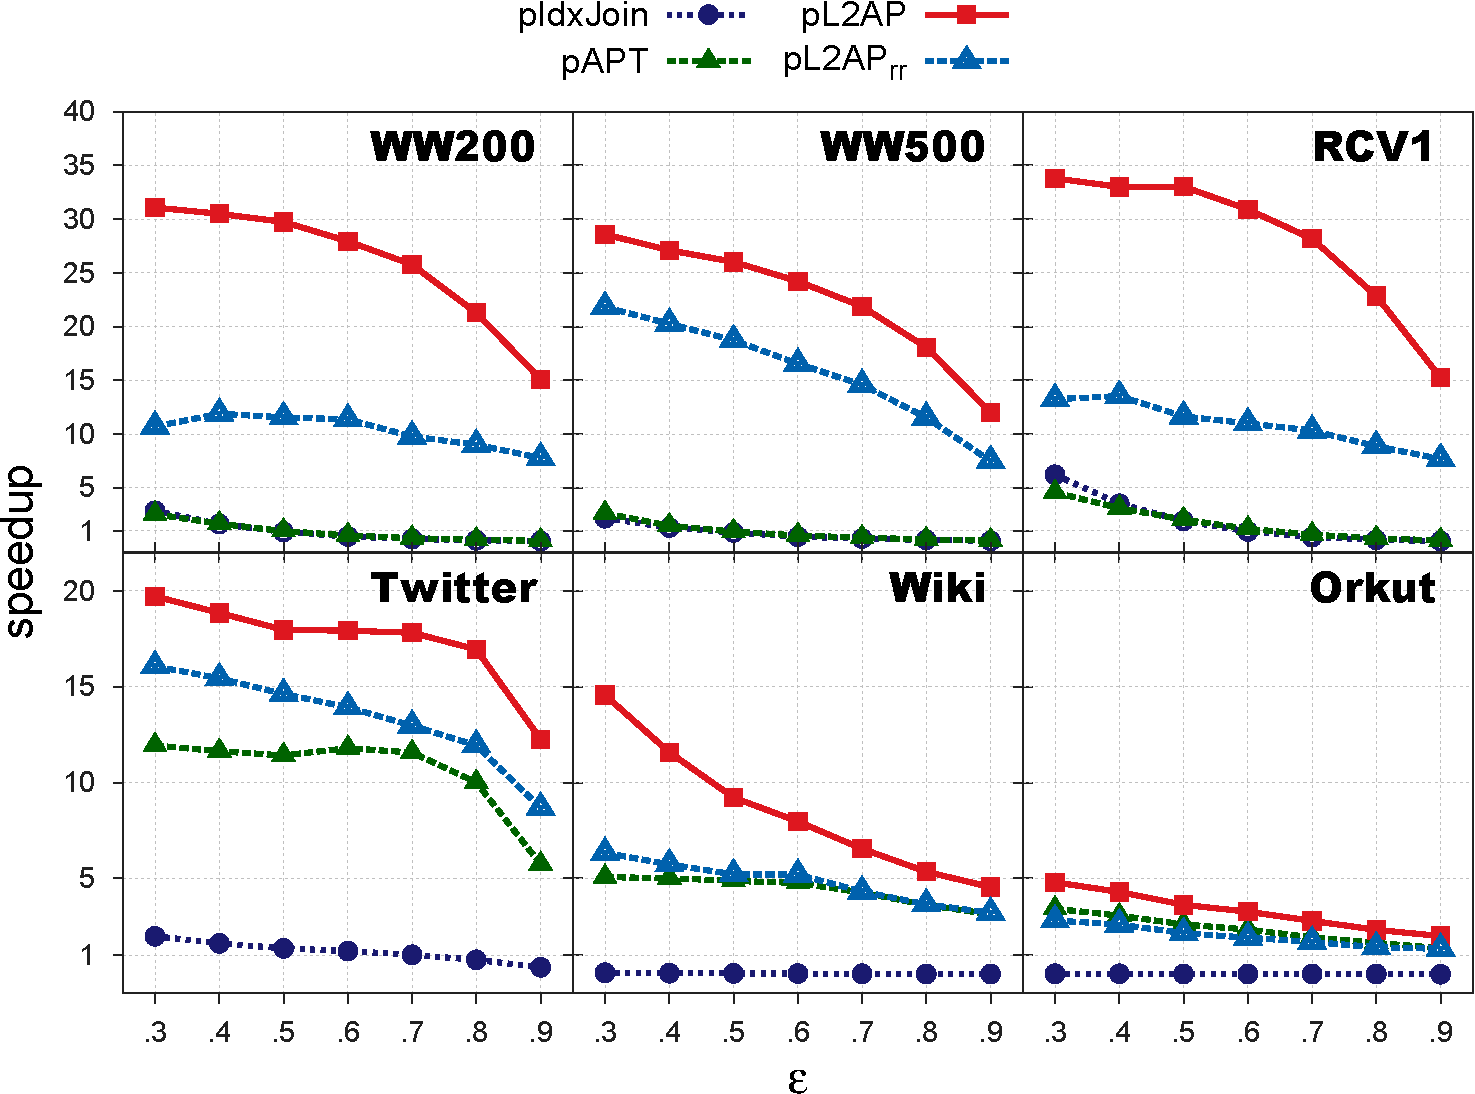
\includegraphics[width=0.85\textwidth]{img/speedup2-nbase.pdf}
  \caption{Speedup comparison of our method against baselines.}
  \label{fig:speedup}
\end{figure}" in main.tex
%%%%%
\appendix
\renewcommand{\thesubsection}{\Alph{subsection}}

\chapter{What Should Be Included in Appendices}\label{apx:appendix1}

Appendices should contain information that is too lengthy to be included in the thesis chapters but further support the conclusions of the thesis. For example, one could include additional experimental results in the form of tables or additional figures. Each appendix should start with a paragraph introducing the items being presented. Additionally, each table or figure should be preceded by a paragraph that explains the data being presented and the conclusions that can be drawn from them. Please note that data already presented in the main thesis should not be repeated in an appendix. One cannot, for example, include the results of an experiment as a figure in the thesis and again as a table in the appendix. One can, however, include detailed results in tables in the appendix and a summary figure in the thesis portraying only the ``best" results.

\section{Subsections in Appendices}\label{apx:appendix1:subsections}

It is possible, and advisable, to use (multiple levels of) subsections in an Appendix. The main Appendix sections may be optionally titled. They will automatically be assigned Appendix A, Appendix B, etc. If a title is present, it will appear on the next line in the appendix and on the same line in the TOC. Sub-sections will be listed in the TOC as A.1, A.2, etc.

Figures, such as \figurename~\ref{fig:nonzero-distr}, should only be referenced in the appendix. The thesis content can point to an appendix but not specifically reference a table or figure in the appendix.

\begin{figure}[!htb]
  \centering
  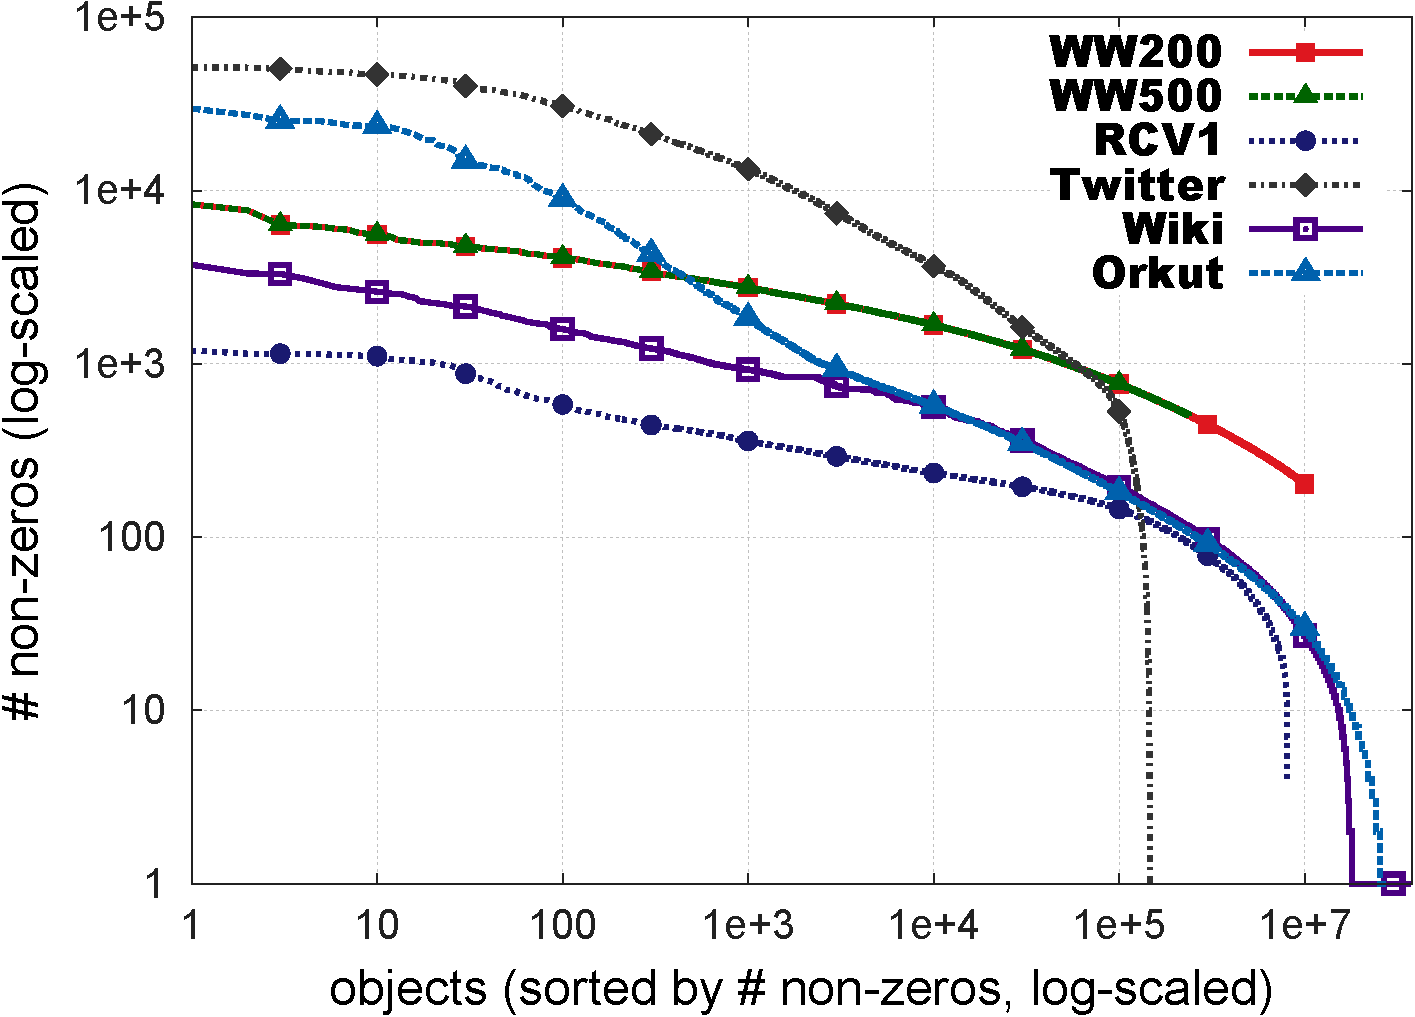
\includegraphics[width=0.6\textwidth]{img/hist-rows.pdf}
  \caption{Distribution of sample non-zeros.}
  \label{fig:nonzero-distr}
\end{figure}


\chapter{Title of Another Appendix}\label{apx:appendix2}

Different appendices should cover unrelated topics. If the appendices are on the same topic, they should just be sub-sections within the same appendix. 

\begin{figure}[tbh]
  \centering
  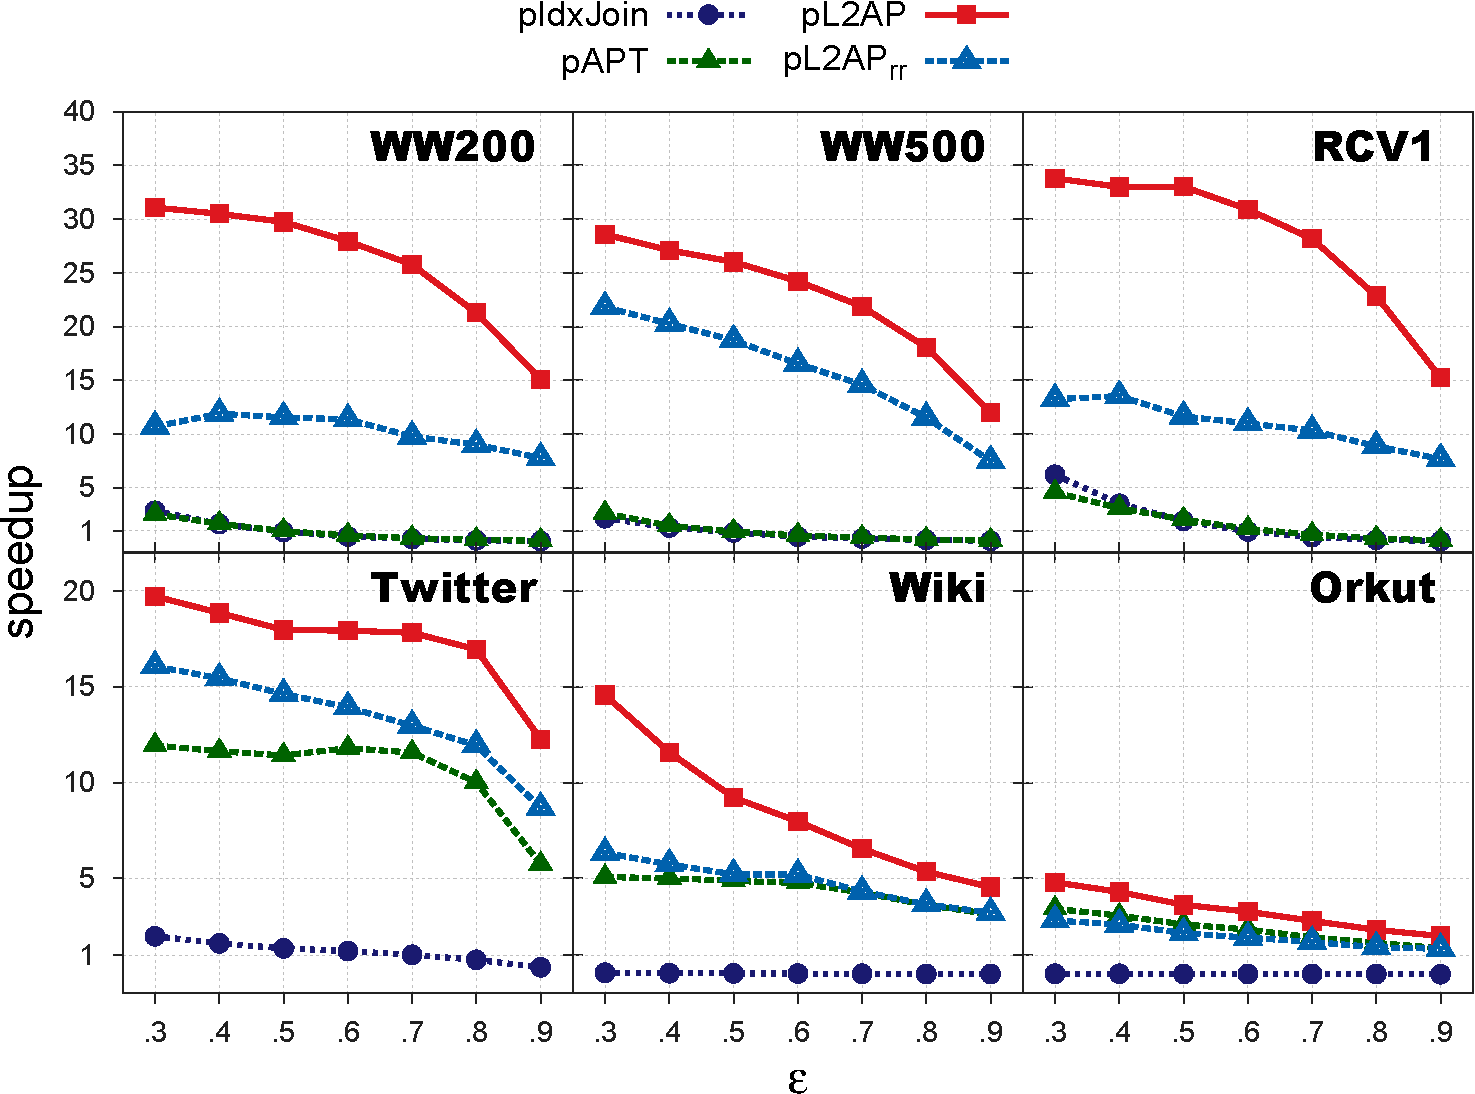
\includegraphics[width=0.85\textwidth]{img/speedup2-nbase.pdf}
  \caption{Speedup comparison of our method against baselines.}
  \label{fig:speedup}
\end{figure}" in main.tex
%%%%%
\appendix
\renewcommand{\thesubsection}{\Alph{subsection}}

\chapter{What Should Be Included in Appendices}\label{apx:appendix1}

Appendices should contain information that is too lengthy to be included in the thesis chapters but further support the conclusions of the thesis. For example, one could include additional experimental results in the form of tables or additional figures. Each appendix should start with a paragraph introducing the items being presented. Additionally, each table or figure should be preceded by a paragraph that explains the data being presented and the conclusions that can be drawn from them. Please note that data already presented in the main thesis should not be repeated in an appendix. One cannot, for example, include the results of an experiment as a figure in the thesis and again as a table in the appendix. One can, however, include detailed results in tables in the appendix and a summary figure in the thesis portraying only the ``best" results.

\section{Subsections in Appendices}\label{apx:appendix1:subsections}

It is possible, and advisable, to use (multiple levels of) subsections in an Appendix. The main Appendix sections may be optionally titled. They will automatically be assigned Appendix A, Appendix B, etc. If a title is present, it will appear on the next line in the appendix and on the same line in the TOC. Sub-sections will be listed in the TOC as A.1, A.2, etc.

Figures, such as \figurename~\ref{fig:nonzero-distr}, should only be referenced in the appendix. The thesis content can point to an appendix but not specifically reference a table or figure in the appendix.

\begin{figure}[!htb]
  \centering
  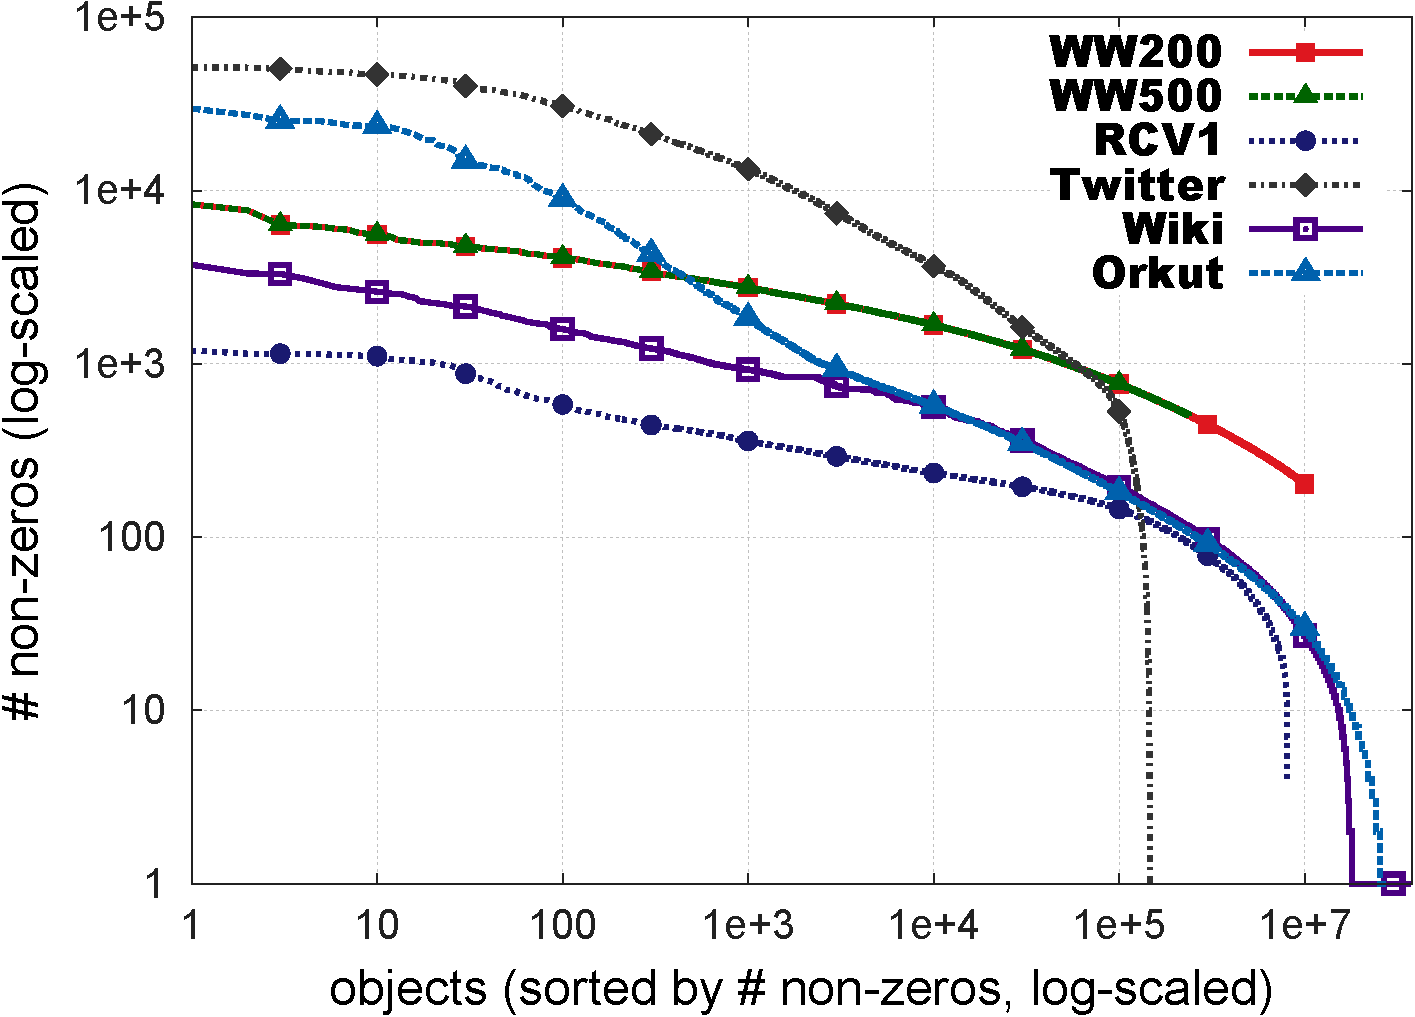
\includegraphics[width=0.6\textwidth]{img/hist-rows.pdf}
  \caption{Distribution of sample non-zeros.}
  \label{fig:nonzero-distr}
\end{figure}


\chapter{Title of Another Appendix}\label{apx:appendix2}

Different appendices should cover unrelated topics. If the appendices are on the same topic, they should just be sub-sections within the same appendix. 

\begin{figure}[tbh]
  \centering
  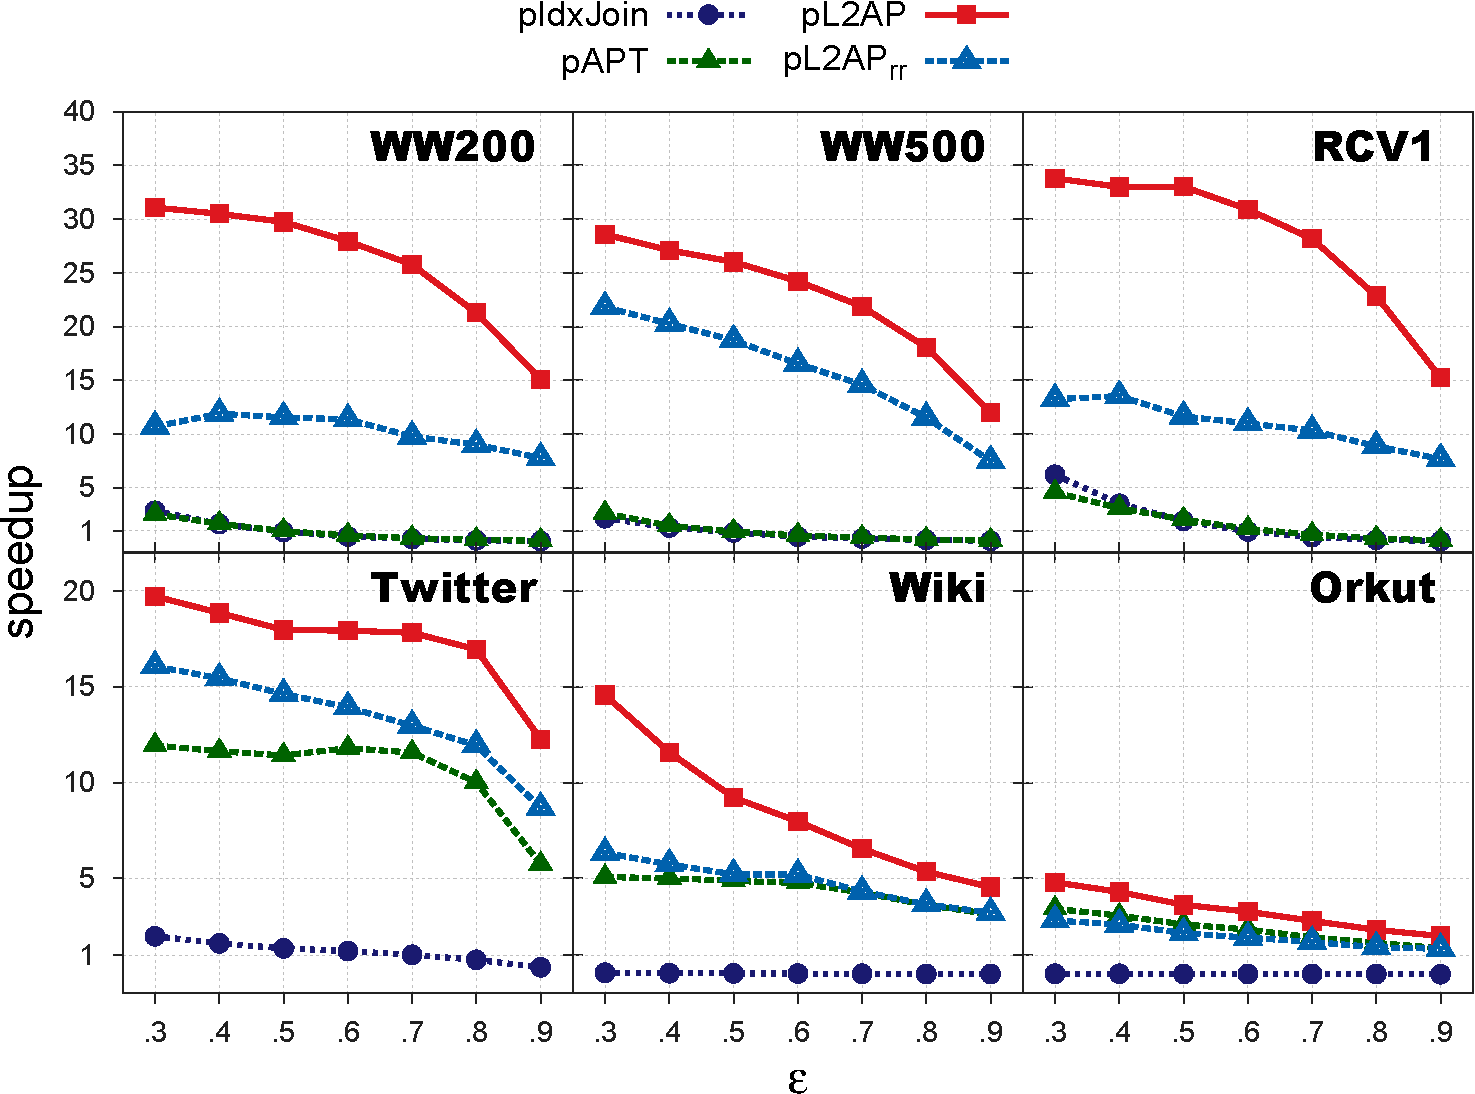
\includegraphics[width=0.85\textwidth]{img/speedup2-nbase.pdf}
  \caption{Speedup comparison of our method against baselines.}
  \label{fig:speedup}
\end{figure}    %% this is optional and can be commented out
\bibliographystyle{ieeetr}
\bibliography{references}
\end{document}
